\documentclass[11pt,twoside,a4paper]{article}

\usepackage{hyperref}
\usepackage{fixltx2e}
\usepackage{amsmath}
\usepackage{amsfonts}
\usepackage{graphicx}
\usepackage{amssymb}
\usepackage{multicol}

% \textsubscript{}
% \textsuperscript{}

\begin{document}
  
  \graphicspath{{img//}}
  
  \title{Maths for Informatics: 4b Geomatry \\Revision Notes}
  \author{Guy Taylor}
  \date{April 2011}
  
  \maketitle
  
  \tableofcontents
  
  \clearpage
  
  \section{Introduction}
    This document is a set of revision notes for the Geomatry for Informatics course at the Univerisy of Edinbugh.
  
  \clearpage
  \section{Mapping}
    If a matrix is arthoginal in \(\mathbb{R}^3\) on can show that \(MM^T = I\) then:
      \begin{description}
        \item[If \(det(m) = 1\)] \hfill \\
          This ia a rotation around some line \(L \in \mathbb{R}^3\) that passes through \(0 (0,0,0)\) at angle \(\alpha\).
          
          If you find the \textit{Eigan Vector} that is a line parralles to \(L\), set it to \((0,0,0)\) and we have the line.
        
        \item[If \(det(m) = -1\)] \hfill \\
          This is a reflection in a plane.
      \end{description}
    
    \begin{tabular}{l|l|l}
      \(x^2+y^2+z^2=1\) & Sphere      & 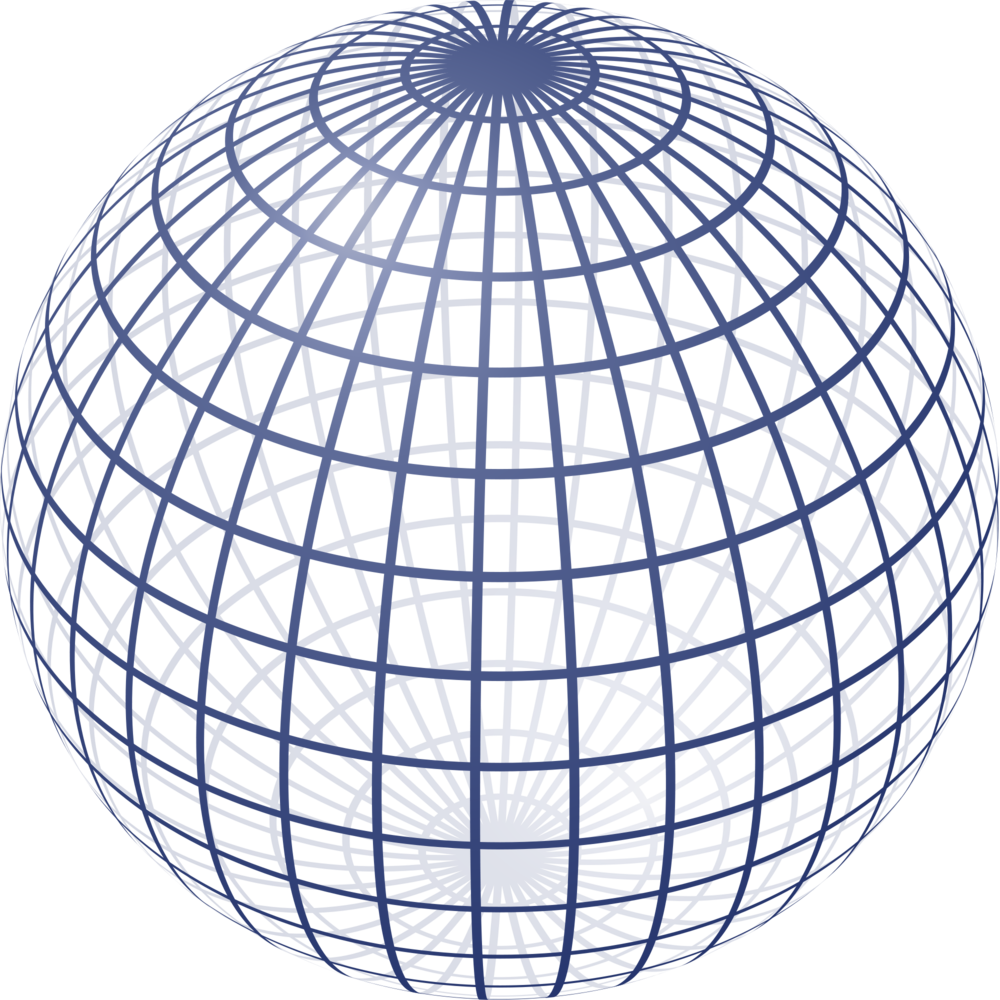
\includegraphics[width=2cm]{Sphere_wireframe_10deg_6r} \\ \hline
      \(x^2+y^2=z^2\)   & Conic       & 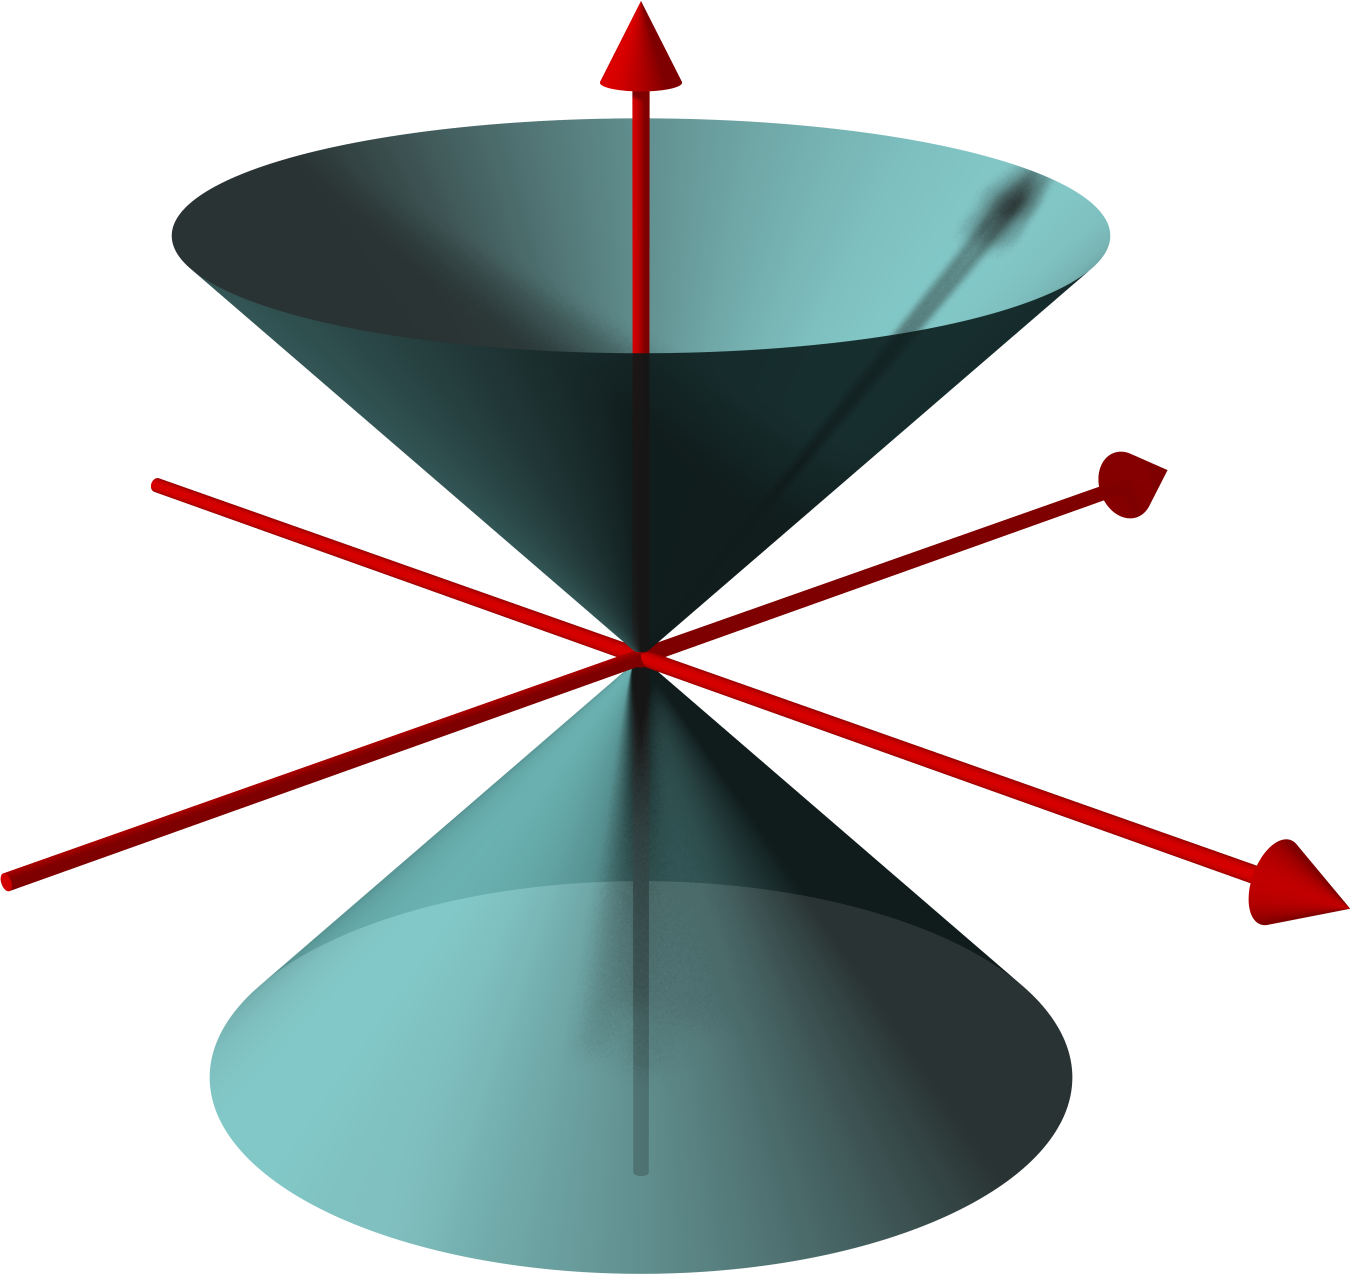
\includegraphics[width=2cm]{DoubleCone} \\ \hline
      \(x^2+y^2=z\)     & Poraboloid  & 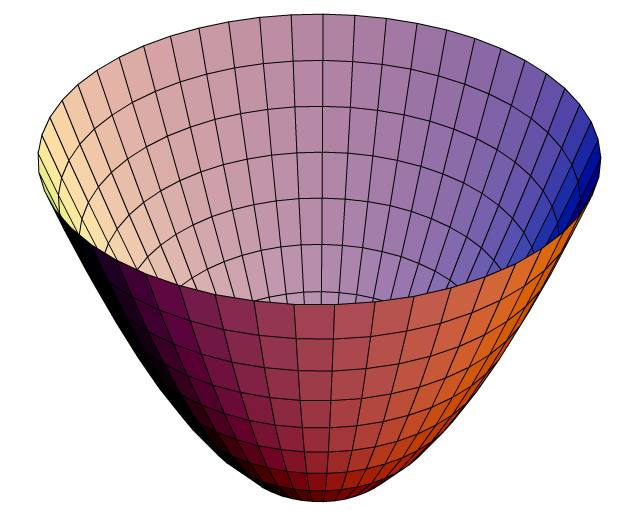
\includegraphics[width=2cm]{Paraboloid_of_Revolution}  \\
    \end{tabular}
    
    \subsection{Example}
      Note: Simmilar to assignment
      \begin{description}
        \item[Question] \hfill \\
          \(
            S:x^2+y^2-z^2=1 \\
            S\subset\mathbb{R}^3 \\
          \)
          If you are given a point and asked to find all lines that pass through it\\
          Hint: There will allways be two
        
        \item[Answer] \hfill \\
        %\begin{multicols}{2}
          \(
            pt(1,1,1) \\*
            P \leq L \leq S \subseteq \mathbb{R}^3 \\
            L = (1+a\alpha, 1+b\alpha, 1+c\alpha) \\
          \)
            \\ Inserted into questions formula \\
          \(
            (1+a\alpha)^2 + (1+b\alpha)^2 + (1+c\alpha)^2 = 1  \forall \alpha \\
          \)
            \\ Expand to\\
          \(
            1+ ... = 1 \\
          \)
            \\ seperate varibles \\
          \(
            \alpha(2a+2b-2c)+\alpha^2(a^2+b^2-c^2) = 0 \\
          \)
            \\ Divide by \alpha \\
          \(
            (2a+2b-2c) = 0 or (a^2+b^2-c^2) = 0 \\
          \)
            \\ let a = 1 (as 1 is modulo all numbers) \\
          \(
            (1,b,c) \\
            1+b^2-c^2 = 0 and 1+b-c=0 \\
            b=0 and c=1 \\
          \)
            \\ Form to a equation \\
          \(
            (1,1,1) + \alpha(1,0,1) \) (are intial point and are new derived point) \\
          
            \\ when a = 0 \\
          \(
            (1,1,1) + \alpha(0,1,1) = :??
          \)
        %\end{multicols}
      \end{description}
  \clearpage
  \bibliography{main}

\end{document}
